\documentclass[a4paper,10pt]{article}
\usepackage[brazilian]{babel}
\usepackage[left=2.5cm,right=2.5cm,top=3cm,bottom=2.5cm]{geometry}
\usepackage{mathtools}
\usepackage{amsthm}
\usepackage{amsmath}
%\usepackage{nccmath}
\usepackage{amssymb}
\usepackage{amsfonts}
\usepackage{physics}
%\usepackage{dsfont}
%\usepackage{mathrsfs}

\usepackage{titling}
\usepackage{indentfirst}

\usepackage{bm}
\usepackage[dvipsnames]{xcolor}
\usepackage{cancel}

\usepackage{xurl}
\usepackage[colorlinks=true]{hyperref}

\usepackage{float}
\usepackage{graphicx}
%\usepackage{tikz}
\usepackage{caption}
\usepackage{subcaption}

%%%%%%%%%%%%%%%%%%%%%%%%%%%%%%%%%%%%%%%%%%%%%%%%%%%

\newcommand{\eps}{\epsilon}
\newcommand{\vphi}{\varphi}
\newcommand{\cte}{\text{cte}}

\newcommand{\N}{\mathbb{N}}
\newcommand{\Z}{\mathbb{Z}}
\newcommand{\Q}{\mathbb{Q}}
\newcommand{\R}{\vb{R}}
\newcommand{\C}{\mathbb{C}}
\renewcommand{\S}{\hat{S}}
%\renewcommand{\H}{\s{H}}

\renewcommand{\a}{\vb{a}}
\newcommand{\nn}{\hat{n}}
\renewcommand{\d}{\dagger}
\newcommand{\up}{\uparrow}
\newcommand{\down}{\downarrow}

\newcommand{\0}{\vb{0}}
%\newcommand{\1}{\mathds{1}}
\newcommand{\E}{\vb{E}}
\newcommand{\B}{\vb{B}}
\renewcommand{\v}{\vb{v}}
\renewcommand{\r}{\vb{r}}
\renewcommand{\k}{\vb{k}}
\newcommand{\p}{\vb{p}}
\newcommand{\q}{\vb{q}}
\newcommand{\F}{\vb{F}}

\newcommand{\s}{\sigma}
%\newcommand{\prodint}[2]{\left\langle #1 , #2 \right\rangle}
\newcommand{\cc}[1]{\overline{#1}}
\newcommand{\Eval}[3]{\eval{\left( #1 \right)}_{#2}^{#3}}

\newcommand{\unit}[1]{\; \mathrm{#1}}

\newcommand{\n}{\medskip}
\newcommand{\e}{\quad \mathrm{e} \quad}
\newcommand{\ou}{\quad \mathrm{ou} \quad}
\newcommand{\virg}{\, , \;}
\newcommand{\ptodo}{\forall \,}
\renewcommand{\implies}{\; \Rightarrow \;}
%\newcommand{\eqname}[1]{\tag*{#1}} % Tag equation with name

\setlength{\droptitle}{-7em}

\theoremstyle{plain}
\newtheorem{theorem}{Teorema}[section]
%\newtheorem{defi}[theorem]{Definição}
\newtheorem{lemma}[theorem]{Lema}
%\newtheorem{corol}[theorem]{Corolário}
%\newtheorem{prop}[theorem]{Proposição}
%\newtheorem{example}{Exemplo}
%
%\newtheorem{inneraxiom}{Axioma}
%\newenvironment{axioma}[1]
%  {\renewcommand\theinneraxiom{#1}\inneraxiom}
%  {\endinneraxiom}
%
%\newtheorem{innerpostulado}{Postulado}
%\newenvironment{postulado}[1]
%  {\renewcommand\theinnerpostulado{#1}\innerpostulado}
%  {\endinnerpostulado}
%
%\newtheorem{innerexercise}{Exercício}
%\newenvironment{exercise}[1]
%  {\renewcommand\theinnerexercise{#1}\innerexercise}
%  {\endinnerexercise}
%
%\newtheorem{innerthm}{Teorema}
%\newenvironment{teorema}[1]
%  {\renewcommand\theinnerthm{#1}\innerthm}
%  {\endinnerthm}
%
\newtheorem{innerlema}{Lema}
\newenvironment{lema}[1]
  {\renewcommand\theinnerlema{#1}\innerlema}
  {\endinnerlema}
%
%\theoremstyle{remark}
%\newtheorem*{hint}{Dica}
%\newtheorem*{notation}{Notação}
%\newtheorem*{obs}{Observação}


\setlength\parindent{0pt}  % noindent in entire file

\usepackage{minted}
\usemintedstyle{vs}
\definecolor{bg}{rgb}{0.85,0.85,0.85}
\setmintedinline{bgcolor=bg}
\newcommand{\python}[1]{\mintinline{python}{#1}}
\usepackage{tcolorbox}
\tcbuselibrary{minted,skins}
\newtcblisting{Python}{
  listing engine=minted,
  colback=bg,
  colframe=black!70,
  listing only,
  minted style=vs,
  minted language=python,
  minted options={texcl=true, fontsize=\scriptsize},
  left=1mm,
}

\renewcommand{\p}{\phantom{+}}
\newcommand{\mchi}{\chi^{\Gamma^0}}
\renewcommand{\c}[1]{\textcolor{red}{#1}}

\title{\Huge{\textbf{Teoria de grupos - Exercício 5}}}
\author{Mateus Marques}

\begin{document}

\maketitle

\section*{Ânion carbonato CO$_3^{2-}$}

Vamos determinar o grupo do CO$_3^{2-}$:
$$
\text{não é linear} \implies \text{eixo }C_{3z} \implies
\text{3 eixos }C_2 \perp C_{3z} \implies
\sigma_h \perp C_{3z} \implies \boxed{ \text{grupo }D_{3h}. }
$$

Os elementos desenhados do grupo $D_{3h}$ estão na Figura \ref{fig:D3h}.
\begin{figure}[H]
\centering
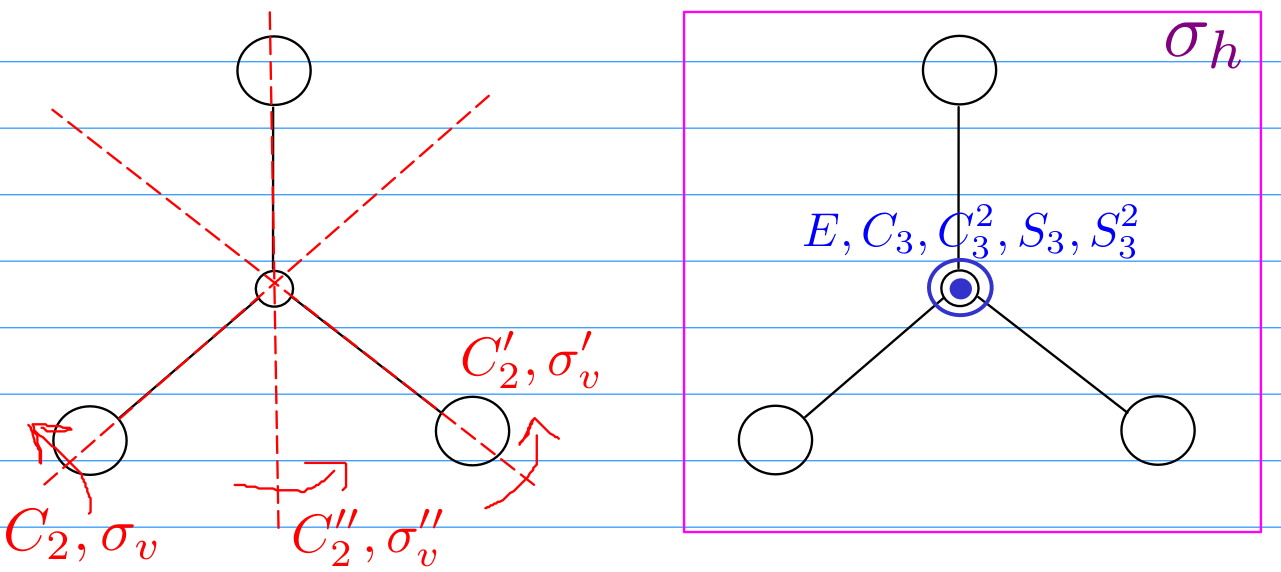
\includegraphics[height=0.32\linewidth]{fig/D3h_my.png}
\caption{Elementos de simetria do grupo $D_{3h}$, correspondente ao ânion carbonato CO$_3^{2-}$.}
\label{fig:D3h}
\end{figure}

\begin{figure}[H]
\centering
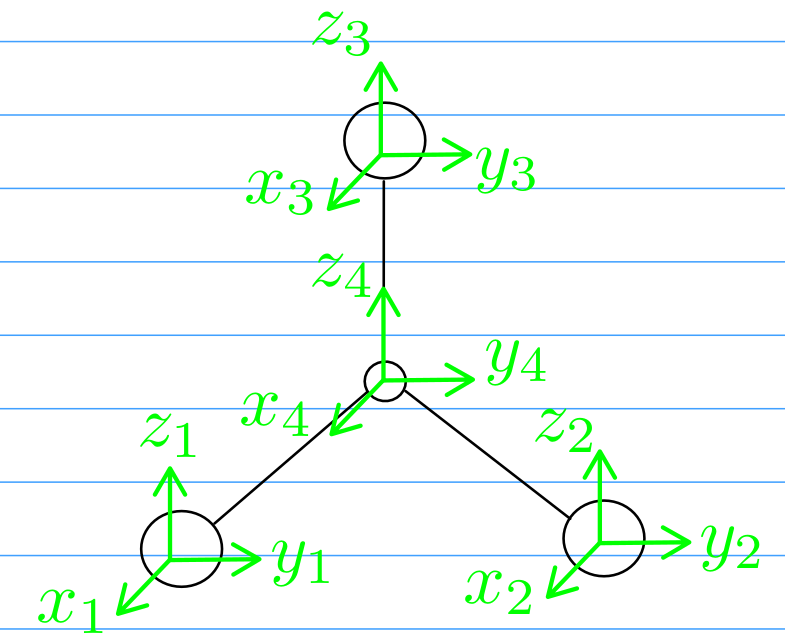
\includegraphics[height=0.32\linewidth]{fig/mov_atom.png}
\caption{As 12 coordenadas do movimento atômico do ânion carbonato CO$_3^{2-}$.}
\label{fig:mov_atom}
\end{figure}

Seja $\Gamma^0$ a representação do movimento atômico do ânion (dimensão 12), seus caracteres são:

\begin{enumerate}
\item $E \implies$ mantém todas as coordenadas. $\chi^{\Gamma^0}(E) = 12$.
\item $2 C_3 \implies$ troca as coordenadas dos oxigênios, enquanto deixa o carbono no lugar.
$$
\begin{pmatrix}
x_4' \\
y_4' \\
z_4' \\
\end{pmatrix}
=
\begin{pmatrix}
\cos2\pi/3 & -\sin2\pi/3 & 0 \\
\sin2\pi/3 &  \cos2\pi/3 & 0 \\
0 & 0 & 1 \\
\end{pmatrix}
\begin{pmatrix}
x_4 \\
y_4 \\
z_4 \\
\end{pmatrix}
\implies \chi^{\Gamma^0}(C_3) = 0.
$$
\item $3 C_2 \implies$ todas as coordenadas mudam, menos os eixos $z$ dos átomos C e O contidos no eixo $C_2$, que mudam de sinal, logo $\chi^{\Gamma^0}(C_2) = -2$.
\item $\sigma_h \implies$ leva as coordenadas $x$ em $-x$, portanto $\chi^{\Gamma^0}(\sigma_h) = 4$.
\item $2 S_3 \implies$ troca as coordenadas dos oxigênios, e mantém as do carbono.
$$
y_4 \to -y_4/2, \quad z_4 \to -z_4/2, \quad x_4 \to -x_4 \implies \mchi(S_3) = -2.
$$
\item $3 \sigma_v \implies$ as coordenadas dos átomos C e O contidos no plano de $\sigma_v$ se transformam
$$
x_3 \to x_3, \quad y_3 \to -y_3, \quad z_3 \to z_3
$$
$$
x_4 \to x_4, \quad y_4 \to -y_4, \quad z_4 \to z_4
$$
Portanto $\mchi(\sigma_v) = 1 - 1 + 1 + 1 - 1 + 1  = 2$.
\end{enumerate}

\begin{table}[H]
\caption{Tabela de caracteres para o grupo $D_{3h}$.}
\centering
\begin{tabular} { |c|c c c c c c | c | c | }
\hline
$D_{3h}$ & $E$ & $2 C_{3}$ & $3 C_{2}$ & $\sigma_h$ & $2 S_3$ & $3 \sigma_v$ & & \\
\hline
$\c{\boxed{A_1'}}$  & $\c{\p1}$ & $\c{\p1}$ & $\c{\p1}$ & $\c{\p1}$ & $\c{\p1}$ & $\c{\p1}$ & & $x^2+y^2$, $z^2$ \\
$\c{\boxed{A_2'}}$  & $\c{\p1}$ & $\c{\p1}$ & $\c{ -1}$ & $\c{\p1}$ & $\c{\p1}$ & $\c{ -1}$ & $\textcolor{blue}{\boxed{R_z}}$ &  \\
$\c{\boxed{3\times E'}}$    & $\c{\p2}$ & $\c{ -1}$ & $\c{\p0}$ & $\c{\p2}$ & $\c{ -1}$ & $\c{\p0}$ & $\textcolor{Orange}{\boxed{(x,y)}}$ & $(x^2-y^2, xy)$ \\
$A_1''$ & $\p1$ & $\p1$ & $\p1$ & $ -1$ & $ -1$ & $ -1$ & & \\
$\c{\boxed{2\times A_2''}}$ & $\c{\p1}$ & $\c{\p1}$ & $\c{ -1}$ & $\c{ -1}$ & $\c{ -1}$ & $\c{\p1}$ & $\textcolor{Orange}{\boxed{z}}$ & \\
$\c{\boxed{E''}}$   & $\c{\p2}$ & $\c{ -1}$ & $\c{\p0}$ & $\c{ -2}$ & $\c{\p1}$ & $\c{\p0}$ & $\textcolor{blue}{(R_x,R_y)}$ & $(xz,yz)$ \\
\hline
\hline
$\Gamma^0$ & $\p12$ & $\p0$ & $ -2$ & $\p4$ & $ -2$ & $\p2$ & & \\
\hline
\end{tabular}
\label{tab:D3h}
\end{table}

Pela tabela de caracteres \ref{tab:D3h}, vemos que
$$
\boxed{ \Gamma^0 = A_1' \oplus A_2' \oplus 3E' \oplus 2A_2'' \oplus E''. }
$$

Para obter os modos vibracionais, basta olhar na tabela \ref{tab:D3h} para saber quais são os de \textcolor{Orange}{translação (em laranja)} e \textcolor{blue}{rotação (em azul)}.
$$
\textcolor{blue}{\Gamma^{rot} = A_2' \oplus E''}
$$
$$
\textcolor{Orange}{\Gamma^{trans} = E' \oplus A_2''}
$$

Como a representação $\Gamma^0$ é decomposta como $\Gamma^0 = \Gamma^{trans} \oplus \Gamma^{rot} \oplus \Gamma^{vib}$, temos que
$$
\boxed{\Gamma^{vib} = A_1' \oplus 2 E' \oplus A_2''.}
$$

Para determinar as transições possíveis no espectro infravermelho, é necessário analisar como as vibrações do sistema alteram o momento de dipolo elétrico. O momento de dipolo é proporcional ao vetor posição, tornando as representações $E' \, (x,y)$ e $A_2'' \, (z)$ da Tabela \ref{tab:D3h} os modos ativos do infravermelho.
$$
\text{modos ativos no infravermelho} =
E' \, (x,y) \text{ e } A_2'' \, (z).
$$

A regra de seleção que governa as transições observáveis no espectro infravermelho envolvendo os estados vibracionais $\psi_{v_i} \to \psi_{v_f}$ é a seguinte:
$$
\Gamma^{\psi_{v_i}} \otimes \Gamma^{\psi_{v_f}} \supset \Gamma^{(x,y)}, \quad
\Gamma^{\psi_{v_i}} \otimes \Gamma^{\psi_{v_f}} \supset \Gamma^{(z)}.
$$

No caso, temos as representações
$$
\Gamma^{(x,y)} = E', \quad \Gamma^{(z)} = A_2''.
$$

O estado final deve corresponder a um dos estados vibracionais, enquanto o estado inicial considerado será o estado fundamental, que é totalmente simétrico no grupo. As únicas transições permitidas são
\begin{figure}[H]
\centering
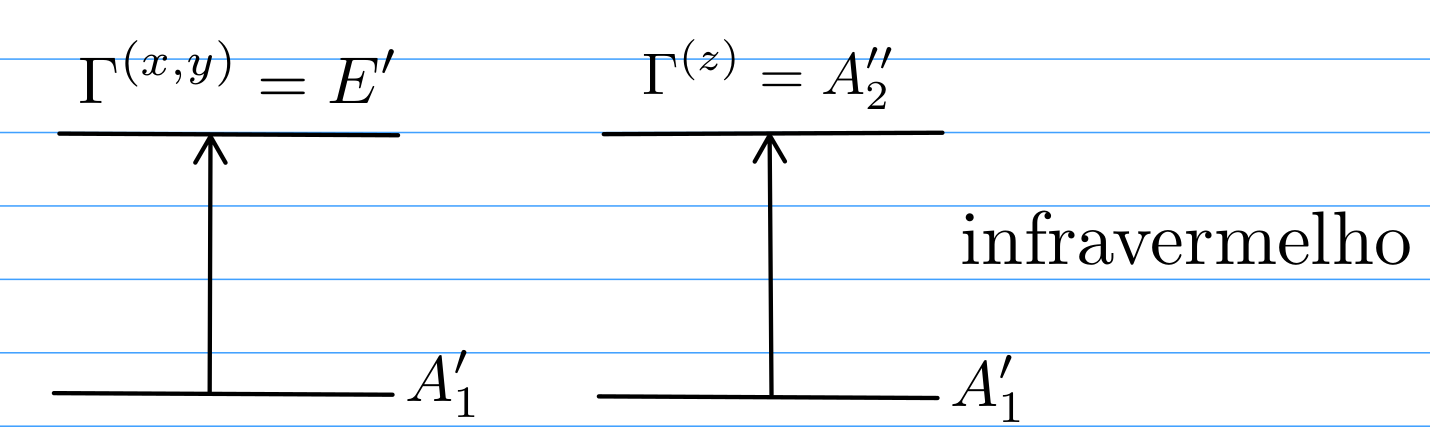
\includegraphics[height=0.15\linewidth]{fig/infravermelho_my.png}
\caption{Transições permitidas no infravermelho.}
\label{fig:infravermelho}
\end{figure}

Vamos analisar o espectro Raman. O efeito Raman envolve transições eletrônicas causadas por um campo elétrico externo, que induz uma polarização no material. Esta polarização está relacionada aos elementos do tensor de polarizabilidade, conforme indicado na tabela de caracteres. Esses elementos podem ser nulos ou não, dependendo dos termos quadráticos. Pelos termos quadráticos da Tabela \ref{tab:D3h}, os modos ativos no Raman são $A_1' (x+y^2, z^2)$ e $E' (x^2-y^2,xy)$.
$$
\text{modos ativos no Raman} = A_1' (x+y^2, z^2) \text{ e } E' (x^2-y^2,xy).
$$

Olhando a Tabela \ref{tab:D3h}, temos
$$
\Gamma^{(x^2+y^2)} = \Gamma^{(z^2)} = A_1', \quad
\Gamma^{(x^2-y^2,xy)} = E', \quad
\Gamma^{(xz,yz)} = E'', \quad
$$

Ao usar as representações das vibrações $\Gamma^{vib} = A_1' \oplus 2 E' \oplus A_2''$ em termos das representações irredutíveis do grupo, obtemos
$$
\underbrace{\Gamma^{vib} \subset \Gamma^{(x^2+y^2)} = \Gamma^{(z^2)} = A_1'}_{\text{permitido}}, \quad
\underbrace{\Gamma^{vib} \subset \Gamma^{(x^2-y^2,xy)} = E'}_{\text{permitido}}, \quad
\underbrace{\Gamma^{vib} \not\subset \Gamma^{(xz,yz)} = E''}_{\text{não permitido}}, \quad
$$

Finalmente, temos os seguintes diagramas para o Raman:
\begin{figure}[H]
\centering
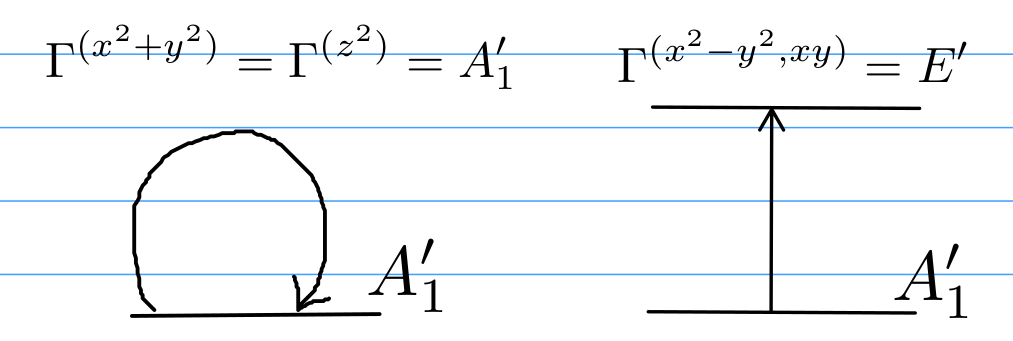
\includegraphics[height=0.15\linewidth]{fig/raman_my.png}
\caption{Transições permitidas no Raman.}
\label{fig:ramn}
\end{figure}

\n


Como a molécula possui três ligações, existem três modos de stretching, e o restante será bending. Na Figura \ref{fig:stretch_bend} temos a esquematização desses modos
\begin{figure}[H]
\centering
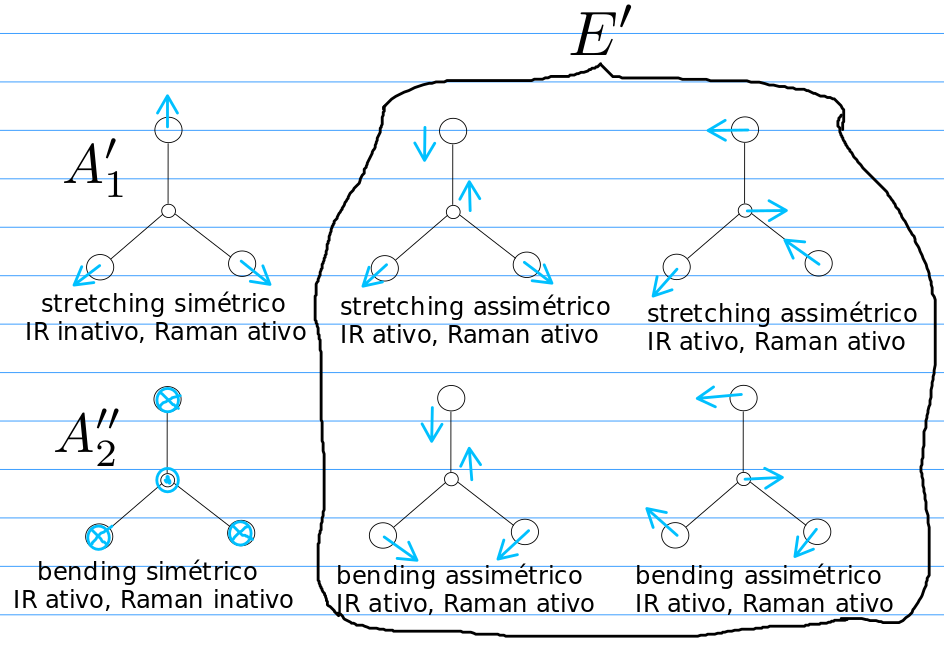
\includegraphics[height=0.4\linewidth]{fig/stretch_bend_my.png}
\caption{Esquematização dos modos de stretching e bending do ânion carbonato.}
\label{fig:stretch_bend}
\end{figure}



\end{document}
